% Options for packages loaded elsewhere
\PassOptionsToPackage{unicode}{hyperref}
\PassOptionsToPackage{hyphens}{url}
%
\documentclass[
  man]{apa6}
\usepackage{amsmath,amssymb}
\usepackage{lmodern}
\usepackage{iftex}
\ifPDFTeX
  \usepackage[T1]{fontenc}
  \usepackage[utf8]{inputenc}
  \usepackage{textcomp} % provide euro and other symbols
\else % if luatex or xetex
  \usepackage{unicode-math}
  \defaultfontfeatures{Scale=MatchLowercase}
  \defaultfontfeatures[\rmfamily]{Ligatures=TeX,Scale=1}
\fi
% Use upquote if available, for straight quotes in verbatim environments
\IfFileExists{upquote.sty}{\usepackage{upquote}}{}
\IfFileExists{microtype.sty}{% use microtype if available
  \usepackage[]{microtype}
  \UseMicrotypeSet[protrusion]{basicmath} % disable protrusion for tt fonts
}{}
\makeatletter
\@ifundefined{KOMAClassName}{% if non-KOMA class
  \IfFileExists{parskip.sty}{%
    \usepackage{parskip}
  }{% else
    \setlength{\parindent}{0pt}
    \setlength{\parskip}{6pt plus 2pt minus 1pt}}
}{% if KOMA class
  \KOMAoptions{parskip=half}}
\makeatother
\usepackage{xcolor}
\usepackage{graphicx}
\makeatletter
\def\maxwidth{\ifdim\Gin@nat@width>\linewidth\linewidth\else\Gin@nat@width\fi}
\def\maxheight{\ifdim\Gin@nat@height>\textheight\textheight\else\Gin@nat@height\fi}
\makeatother
% Scale images if necessary, so that they will not overflow the page
% margins by default, and it is still possible to overwrite the defaults
% using explicit options in \includegraphics[width, height, ...]{}
\setkeys{Gin}{width=\maxwidth,height=\maxheight,keepaspectratio}
% Set default figure placement to htbp
\makeatletter
\def\fps@figure{htbp}
\makeatother
\setlength{\emergencystretch}{3em} % prevent overfull lines
\providecommand{\tightlist}{%
  \setlength{\itemsep}{0pt}\setlength{\parskip}{0pt}}
\setcounter{secnumdepth}{-\maxdimen} % remove section numbering
% Make \paragraph and \subparagraph free-standing
\ifx\paragraph\undefined\else
  \let\oldparagraph\paragraph
  \renewcommand{\paragraph}[1]{\oldparagraph{#1}\mbox{}}
\fi
\ifx\subparagraph\undefined\else
  \let\oldsubparagraph\subparagraph
  \renewcommand{\subparagraph}[1]{\oldsubparagraph{#1}\mbox{}}
\fi
\newlength{\cslhangindent}
\setlength{\cslhangindent}{1.5em}
\newlength{\csllabelwidth}
\setlength{\csllabelwidth}{3em}
\newlength{\cslentryspacingunit} % times entry-spacing
\setlength{\cslentryspacingunit}{\parskip}
\newenvironment{CSLReferences}[2] % #1 hanging-ident, #2 entry spacing
 {% don't indent paragraphs
  \setlength{\parindent}{0pt}
  % turn on hanging indent if param 1 is 1
  \ifodd #1
  \let\oldpar\par
  \def\par{\hangindent=\cslhangindent\oldpar}
  \fi
  % set entry spacing
  \setlength{\parskip}{#2\cslentryspacingunit}
 }%
 {}
\usepackage{calc}
\newcommand{\CSLBlock}[1]{#1\hfill\break}
\newcommand{\CSLLeftMargin}[1]{\parbox[t]{\csllabelwidth}{#1}}
\newcommand{\CSLRightInline}[1]{\parbox[t]{\linewidth - \csllabelwidth}{#1}\break}
\newcommand{\CSLIndent}[1]{\hspace{\cslhangindent}#1}
\ifLuaTeX
\usepackage[bidi=basic]{babel}
\else
\usepackage[bidi=default]{babel}
\fi
\babelprovide[main,import]{english}
% get rid of language-specific shorthands (see #6817):
\let\LanguageShortHands\languageshorthands
\def\languageshorthands#1{}
% Manuscript styling
\usepackage{upgreek}
\captionsetup{font=singlespacing,justification=justified}

% Table formatting
\usepackage{longtable}
\usepackage{lscape}
% \usepackage[counterclockwise]{rotating}   % Landscape page setup for large tables
\usepackage{multirow}		% Table styling
\usepackage{tabularx}		% Control Column width
\usepackage[flushleft]{threeparttable}	% Allows for three part tables with a specified notes section
\usepackage{threeparttablex}            % Lets threeparttable work with longtable

% Create new environments so endfloat can handle them
% \newenvironment{ltable}
%   {\begin{landscape}\centering\begin{threeparttable}}
%   {\end{threeparttable}\end{landscape}}
\newenvironment{lltable}{\begin{landscape}\centering\begin{ThreePartTable}}{\end{ThreePartTable}\end{landscape}}

% Enables adjusting longtable caption width to table width
% Solution found at http://golatex.de/longtable-mit-caption-so-breit-wie-die-tabelle-t15767.html
\makeatletter
\newcommand\LastLTentrywidth{1em}
\newlength\longtablewidth
\setlength{\longtablewidth}{1in}
\newcommand{\getlongtablewidth}{\begingroup \ifcsname LT@\roman{LT@tables}\endcsname \global\longtablewidth=0pt \renewcommand{\LT@entry}[2]{\global\advance\longtablewidth by ##2\relax\gdef\LastLTentrywidth{##2}}\@nameuse{LT@\roman{LT@tables}} \fi \endgroup}

% \setlength{\parindent}{0.5in}
% \setlength{\parskip}{0pt plus 0pt minus 0pt}

% Overwrite redefinition of paragraph and subparagraph by the default LaTeX template
% See https://github.com/crsh/papaja/issues/292
\makeatletter
\renewcommand{\paragraph}{\@startsection{paragraph}{4}{\parindent}%
  {0\baselineskip \@plus 0.2ex \@minus 0.2ex}%
  {-1em}%
  {\normalfont\normalsize\bfseries\itshape\typesectitle}}

\renewcommand{\subparagraph}[1]{\@startsection{subparagraph}{5}{1em}%
  {0\baselineskip \@plus 0.2ex \@minus 0.2ex}%
  {-\z@\relax}%
  {\normalfont\normalsize\itshape\hspace{\parindent}{#1}\textit{\addperi}}{\relax}}
\makeatother

% \usepackage{etoolbox}
\makeatletter
\patchcmd{\HyOrg@maketitle}
  {\section{\normalfont\normalsize\abstractname}}
  {\section*{\normalfont\normalsize\abstractname}}
  {}{\typeout{Failed to patch abstract.}}
\patchcmd{\HyOrg@maketitle}
  {\section{\protect\normalfont{\@title}}}
  {\section*{\protect\normalfont{\@title}}}
  {}{\typeout{Failed to patch title.}}
\makeatother

\usepackage{xpatch}
\makeatletter
\xapptocmd\appendix
  {\xapptocmd\section
    {\addcontentsline{toc}{section}{\appendixname\ifoneappendix\else~\theappendix\fi\\: #1}}
    {}{\InnerPatchFailed}%
  }
{}{\PatchFailed}
\keywords{keywords\newline\indent Word count: X}
\DeclareDelayedFloatFlavor{ThreePartTable}{table}
\DeclareDelayedFloatFlavor{lltable}{table}
\DeclareDelayedFloatFlavor*{longtable}{table}
\makeatletter
\renewcommand{\efloat@iwrite}[1]{\immediate\expandafter\protected@write\csname efloat@post#1\endcsname{}}
\makeatother
\usepackage{lineno}

\linenumbers
\usepackage{csquotes}
\usepackage{graphicx}
\ifLuaTeX
  \usepackage{selnolig}  % disable illegal ligatures
\fi
\IfFileExists{bookmark.sty}{\usepackage{bookmark}}{\usepackage{hyperref}}
\IfFileExists{xurl.sty}{\usepackage{xurl}}{} % add URL line breaks if available
\urlstyle{same} % disable monospaced font for URLs
\hypersetup{
  pdftitle={Decomposing fish species distribution to identify characteristic spatial patterns},
  pdfauthor={First Author1 \& Second author1,2},
  pdflang={en-EN},
  pdfkeywords={keywords},
  hidelinks,
  pdfcreator={LaTeX via pandoc}}

\title{Decomposing fish species distribution to identify characteristic spatial patterns}
\author{First Author\textsuperscript{1} \& Second author\textsuperscript{1,2}}
\date{}


\shorttitle{EOF}

\authornote{

Add authornote

Correspondence concerning this article should be addressed to First Author, Postal address. E-mail: \href{mailto:my@email.com}{\nolinkurl{my@email.com}}

}

\affiliation{\vspace{0.5cm}\textsuperscript{1} Institution 1\\\textsuperscript{2} Institution 2}

\abstract{%
Here goes the abstract
}



\begin{document}
\maketitle

Species phenology --\textgreater{} major uncertainty

While key in understanding species life cycle and has major ecological and conservation implications.

\hypertarget{methods}{%
\section{Methods}\label{methods}}

\hypertarget{species-data-and-model-outputs}{%
\subsection{Species, data and model outputs}\label{species-data-and-model-outputs}}

\hypertarget{case-studies}{%
\subsubsection{Case studies}\label{case-studies}}

We selected sole and sea bass in the Bay of Biscay as well as Hake in both the Bay of Biscay and the Celtic Sea as case studies. These three case studies are selected as they all benefit from scientific and expert knowledge regarding their phenology in order to validate the results of their analysis.

Sole of the Bay of Biscay reproduce.

Sea bass in the Bay of Biscay is .

Hake in the Bay of Biscay and in the Celtic Sea is considered as one single stock. Still, there is question about the

To map species distribution, we filtered the data from several trawler fleets from 2008 to 2018.

\hypertarget{data}{%
\subsubsection{Data}\label{data}}

\hypertarget{model-and-model-outputs-format}{%
\subsubsection{Model and model outputs format}\label{model-and-model-outputs-format}}

\hypertarget{decomposing-model-outputs}{%
\subsection{Decomposing model outputs}\label{decomposing-model-outputs}}

\hypertarget{eof}{%
\subsubsection{EOF}\label{eof}}

Empirical Orthogonal Functions is a method that has been developped by Lorenz (1956) for weather forecasting applications. The original aim of the technic was to deduce from a set of spatio-temporal maps a smaller set of maps that best describe and summarise the spatio-temporal process of interest. The main idea was to define the spatio-temporal process \(S(x,t)\) as a linear combination of spatial patterns \(p_m\) (named EOF) each related to temporal indices \(\alpha_m(t)\) (Equation \ref{eq:EOF} - \(x\in[\![1,N]\!],t\in[\![1,T]\!]\)). These temporal indices indicate when the spatio-temporal process is distributed following their related spatial pattern.

\begin{align} \label{eq:EOF}
S(x,t)=\sum_{m=1}^M \alpha_m(t) \cdot p_m(x) + r^M(x,t)
\end{align}

where \(r^M(x,t)\) is the residual variation not captured by the \(M\) modes of variation \(\alpha_m(t) \cdot p(m,x)\).

To estimate the temporal components \(\alpha_m(t)\) and the spatial patterns \(p(m,x)\), some criteria need to be set. A natural choice is to minimize the residual variation to best capture the variability \(S(x,t)\) (i.e.~\(R^M=\sum^M_{m=1}(r^M_m)^2\) is minimized) and set orthogonal constraints between the modes of variability so that each mode is the `best' representation of variability from a statistical point of view (Equations \ref{eq:Orthog1}, \ref{eq:Orthog2}). This last criteria is further discussed in the discussion.

\begin{align}
\label{eq:Orthog1}
\sum^N_{x=1} p_m(x) \cdot p_j(x) = \delta_{mj} \equiv \Bigg \{ \begin{array}{lll}1 & \text { if } & m=j \\ 0 & \text { if } & m \neq j\end{array}
\end{align}

\begin{align}
\label{eq:Orthog2}
T \cdot \overline{p_m^* p_j^*} = a_m \delta_{mj}
\end{align}

with \(a_m \geq a_{m+1} \geq 0\), \(\overline{( \ )}\) denoting the time average and \(( \ )^*\) a departure from the time average.

Let's write these equations in matrix terms by introducing the \(T \times N\) matrix \(\mathbf{S}\), \(\mathbf{S}^*\), \(\mathbf{Q}\), \(\mathbf{Q}^*\). They respectively refer to \(S(x,t)\), \(S^*(x,t)\), \(\alpha_m(t)\) and \(\alpha_m^*(t)\). We denote \(\mathbf{Y}\) is a square matrix of order \(N\) with elements \(p_{m}(x)\) (NEED TO CHECK). Then, the problem can be reformulated as:

\begin{align}
& \mathbf{S}=\mathbf{QY} \\
& \mathbf{YY}^T=\mathbf{I} \\
& {\mathbf{Q}^{*}}^T\mathbf{Q} = \mathbf{D}
\end{align}

with \(\overline{(\ )}\) the transpose, \(\mathbf{I}\) the identity, \(\mathbf{D}\) a diagonal matrix with diagonal being equal to \(a_m / T\).

Finally, by introducing \(A \equiv {Q^*}^T Q^*\) (whose elements are proportionnal to the covariance of \(\alpha_m(t)\)), we can rewrite these equations as:

\begin{align}
\label{eq:Diag}
\mathbf{YAY}^T=\mathbf{D}
\end{align}

This is a standard ``eigenvalue-eigenvector'' problem. As a consequence, a link can be done with standard multivariate analysis such as PCA. Thus, in addition to the spatial patterns (and the related temporal components) that appear in the EOF formulations (Equation \ref{eq:EOF}) and that can be obtained by diagonalysing the problem in Equation \ref{eq:Diag}, additionnal analysis can be performed to obtain similar visualisation as in PCA (e.g.~plot of individuals and variables) possibly coupled with standard clustering analysis.

\hypertarget{link-with-pca}{%
\subsubsection{Link with PCA}\label{link-with-pca}}

In this representation (Equation \ref{eq:Diag}), \(\mathbf{Y}^T=X\) is the matrix of \(p_{m}(x)\) which are the eigen-vectors in PCA analysis, \(A\) is the covariance matrix of the centered predictions \(\mathbf{S}^*\) (TO CHECK) and \(\mathbf{D}\) is the diagonal matrix of the eigen-values.

Often, this equation cannot be resolved as the A matrix is not diagonalisable (when there are more spatial locations than time-steps). Then, it is required to pass through singular value decomposition to get the eigen-values and eigen-vectors of \(A\).

Singluar value decomposition (svd) express a matrix \(\mathbf{X}\) as a decomposition of 3 other matrices:

\(\mathbf{X}=\mathbf{U} \mathbf{\Lambda} \mathbf{V}^{\prime}\) with \(\mathbf{U U}^{\prime}=\mathbf{U}^{\prime} \mathbf{U}=\mathbf{I}\) and \(\mathbf{V V}^{\prime}=\mathbf{V}^{\prime} \mathbf{V}=\mathbf{I}\).

From these expressions, we can demonstrate that \(\mathbf{XX}^{\prime} = \mathbf{V}^{\prime} \mathbf{\Lambda}^2 \mathbf{V}\) with \(\mathbf{\Lambda}^2\) the eigen-values and \(\mathbf{V}\) the eigen-vectors of the covariance matrix \(\mathbf{XX}^{\prime}\). The eigen-values and eigen-vectors of the covariance matrix \(\mathbf{A}\) where obtained from svd and allowed to performed the same analysis as in standard PCA (more precisely a PCA is a svd on centered or centered-reduced data if the PCA is normalized).

\hypertarget{representing-variables-and-individuals}{%
\subsubsection{Representing variables and individuals}\label{representing-variables-and-individuals}}

Then, we analyse the spatio-temporal model outputs by presenting the spatial patterns \(p_m(x)\) (i.e.~the eigen-vectors) which are in the matrix \(\mathbf{X}=\mathbf{V}\). These can be seen as maps that structure the actual process \(\mathbf{S}\) (Cf. Figure\ldots) or alternatively as standard variable plot as in classical PCA analysis (Cf. Figure\ldots).

The temporal index \(\alpha_m(t)\) are the projection matrix \(\mathbf{S}^*\) onto the EOF basis function \(\mathbf{V}\) i.e.~\(A=\mathbf{S}^*\mathbf{X}=\mathbf{U} \mathbf{\Lambda}\). These can be either seen as time series (Cf. Figure\ldots) or as a classical plot of individuals on the first components of the PCA (Cf. Figure\ldots).

When confronted together, the spatial representations and the related temporal indices inform how the spatial patterns vary in time.

\textbf{FIGURE: LINK BETWEEN EOF AND PCA}

Spectral analysis: - \url{https://bookdown.org/rdpeng/timeseriesbook/spectral-analysis.html} - \url{https://math.mcmaster.ca/~bolker/eeid/2010/Ecology/Spectral.pdf}

\hypertarget{results}{%
\section{Results}\label{results}}

\hypertarget{strong-seasonnal-patterns}{%
\subsection{Strong seasonnal patterns}\label{strong-seasonnal-patterns}}

--\textgreater{} 2 first capture around 20\% each and often very seasonnal

--\textgreater{} seasonnal PC, coincide with reproduction ecology --\textgreater{} result from migration patterns ?

--\textgreater{} Northward move for Hake and Sole

\hypertarget{identifying-seasons-and-functional-zones}{%
\subsection{Identifying seasons and functional zones}\label{identifying-seasons-and-functional-zones}}

--\textgreater{} result of clustering on temporal indices and related groups

High inter-annual stability, no confusion between month/cluster

--\textgreater{} related spatial patterns

\hypertarget{discussion}{%
\section{Discussion}\label{discussion}}

\begin{itemize}
\item
  Northward move --\textgreater{} climate change ?
\item
  EOM ? Constraints to build the maps
\end{itemize}

--\textgreater{} `best' representation of variability from a statistical point of view = `second basis function should be spatially uncorrelated with the first, and this is equivalent to the requirement of spatial orthogonality'

(Lorenz, 1956; Randall, 2003)

(Monahan, Fyfe, Ambaum, Stephenson, \& North, 2009)

\newpage

\hypertarget{references}{%
\section{References}\label{references}}

\begingroup
\setlength{\parindent}{-0.5in}
\setlength{\leftskip}{0.5in}

\hypertarget{refs}{}
\begin{CSLReferences}{1}{0}
\leavevmode\vadjust pre{\hypertarget{ref-lorenz1956empirical}{}}%
Lorenz, E. N. (1956). \emph{Empirical orthogonal functions and statistical weather prediction} (Vol. 1). Massachusetts Institute of Technology, Department of Meteorology Cambridge.

\leavevmode\vadjust pre{\hypertarget{ref-monahan2009empirical}{}}%
Monahan, A. H., Fyfe, J. C., Ambaum, M. H., Stephenson, D. B., \& North, G. R. (2009). Empirical orthogonal functions: The medium is the message. \emph{Journal of Climate}, \emph{22}(24), 6501--6514.

\leavevmode\vadjust pre{\hypertarget{ref-randall2003empirical}{}}%
Randall, D. (2003). Empirical orthogonal functions. \emph{Dept. Atmosph. Sci., Colorado State Univ., CO, USA}.

\end{CSLReferences}

\endgroup

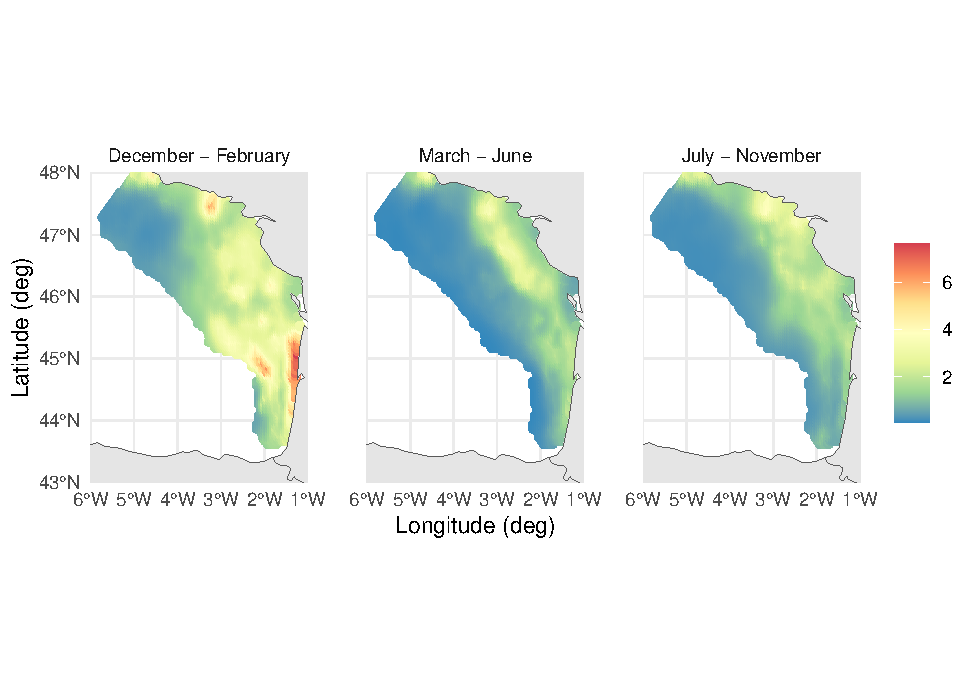
\includegraphics{paper_4_files/figure-latex/SM plot-1.pdf}


\end{document}
